\documentclass[10pt]{article}
\usepackage{helvet}
\usepackage{graphicx}
\newcommand\tab[1][1cm]{\hspace*{#1}}
\usepackage[left=1.1cm,top=1.2cm,right=1.1cm,bottom=1.2cm]{geometry}
\usepackage{tabularx}
\usepackage{placeins}
\usepackage{longtable}
\usepackage{enumitem}
\renewcommand{\familydefault}{\sfdefault}
\usepackage{titling}
\setlength{\droptitle}{-3em} 
\begin{document}
\title{%
	Using Evolutionary Algorithms to Solve Sudoku Problems
	}
\author{640034510}
\date{March 05, 2018}
\maketitle

\section{Introduction}
% Implemented a generational evolutionary algorithm with tournament based selection
\paragraph{•}
The Sudoku puzzle is a combinatorial number placement problem where the player must fill a partially completed nine by nice grid with sets of the numbers one to nine. These numbers must be placed in a way such that each row, column, and three by three sub grid contains a unique set. Due to this constraint on the placement of numbers, Sudoku proves to be a NP-complete problem which makes it impracticable to solve using a direct method. Instead a heuristic search method must be applied to the problem, of which the genetic algorithm metaheuristic is highlighted in this report. Inspired by the biological process of Meiosis, genetic algorithms encode potential solutions as chromosomes which undergo a series of genetic operators to produce offspring. Over successive generations of offspring, the average fitness of the population should increase until the final solution is found, or the population has converged to some local maxima.
\section{Design}
\subsection{Solution Space and Representation}
\paragraph{•}
The solution space for an empty nine by nine Sudoku grid is vast, with an approximate $6.67\cdot10^{21}$ possible grids. As the number of clues given in a Sudoku puzzle increases then the possible solution space decreases but still remains large. To further reduce the size of the solution space, it was decided that all solutions must have valid rows. That is, all rows of a candidate solution must contain some permutation of the set of numbers one to nine. All subsequent operators on the population must therefore conserve this rule to ensure that the search space remains reduced and errant solutions do not enter the population. Solutions are represented as a one-dimensional list of integers, the length of which is set to the number of spaces in the Sudoku grid. This representation was chosen as it makes representing rows, columns, and grids within the solution trivial. Additionally, this representation allows for genetic operators, described below, to be applied to chromosomes in an way analogous to that of their biological counterparts.

\subsection{Population Initialisation}
\paragraph{•}
The population is initialised by copying the two-dimensional grid into a one dimensional chromosome, preserving the pre-set numbers and setting zero for spaces which are blank. For each row in the grid, the set of the existing numbers is calculated and the blanks are filled from the inverse of this set, creating rows which are a permutation of the numbers one to nine.

\subsection{Fitness Function}
\paragraph{•}
The success state of a Sudoku puzzle is when the contents of every row, column, and box are each a permutation of the numbers of the numbers one to nine. Therefore, the fitness function first calculates the sum of the number of unique digits in each column and box. This number is then normalized in the range of zero and one by dividing it by the maximum number of unique digits in all rows and columns. In the case of a nine by nine Sudoku grid, the maximum number of unique digits in the rows and columns is 162. Rows have been excluded from this metric as all solutions already have valid rows from initialisation. By only including rows and columns in the metric, any positive change to the fitness of a row or column will have a greater impact on the overall fitness score of the solution.

\subsection{Selection and Replacement}
\paragraph{•}
To select parents to produce offspring, binary tournament selection is used. This operator picks two solutions from the population and compares their fitness functions. The solution with the greatest fitness function is chosen to be a parent used to produce the subsequent generation. A binary tournament selector is used as it reduces selection pressure which is important because of the amount of local maximum present within a Sudoku problem. By allowing less optimal solutions to affect the subsequent generation, a wider diversity of solutions will be present which may overcome a local maximum. Replacement is done using a pure generational scheme, where the children replace the existing population entirely in the subsequent generation. This was to provide an answer faster than a similar steady state algorithm and to decrease selection pressure between generations.
\subsection{Crossover Function}
\paragraph{•}
The crossover function used is a row-orientated n-point swap operator which produces two children from two parents. One child, picked at random, is assigned the first row of parent one while the other receives the first row of parent two. This is repeated for each row in a parent has until both children comprise of the shuffled rows of both parents. This operator was chosen to promote diversity within the offspring of the current generation and to overcome local maxima. It was felt that only swapping one row would favour solutions which would arise from combinations current rows and would prevent the algorithm from keeping diverse individuals in the population.
\subsection{Mutation Function}
\paragraph{•}
The mutation function chosen is a single swap mutator which ensures that the resultant mutant retains valid row permutations. To do this, the mutator first picks a row within the grid and then two genes within that. If the two selected indexes are distinct then the genes contained within are swapped. In this way, the diversity of possible candidate solutions is increased and may help to overcome a local maximum while preserving permutations. The chance that a gene will be mutated is set to 0.5 such that half of all chromosomes within a population will undergo the mutation. This was chosen to ensure mutations occur while still preserving some strong solutions to increase selection pressure.


\subsection{Termination Criteria}
\paragraph{•}
There are three termination criteria that halt the operation of the genetic algorithm. The first is when an optimal solution, one where the fitness function equals one, has been found as simply no more generations need to be produced. The second is when a thousand generations have been reached which allows time for small population sizes to reach a solution while not being overly long. This number is reduced to 200 in the case of a population size of 10000 due to the expectation that an optimal solution should be reached before. Finally, if there has been not change to the best solution in a population for 200 generations then the runtime is terminated. This shows that a local maximum has been reached and the population has subsequently stagnated.

\section{Experiments}
\paragraph{•}
Three experiments were designed and run to test the effect that various genetic operators have on a population. These genetic operators were tested at a range of population sizes and on increasingly harder Sudoku problems. To control the number of variables in each experiment and to facilitate comparison between them, the mutation chance was set to 0.5. Additionally, the crossover rate is set to one, such that every pair of parents will produce a distinct pair of offspring. All other variables, such as tournament size, are set as described in the design section. Each experiment was run on three Sudoku puzzles of ascending difficulty called Grid 1, Grid 2, and Grid 3 respectively. A range of population sizes were tested, with populations set to 10, 100, 1000, and 10000 individuals. The genetic algorithm was then run on each grid five times to measure the average best fitness for each population size.

\paragraph{•}Three modifications to the genetic operators were tested, the first of which was to add an elitism operator to when a generation is replaced with its offspring. The elitism operator first selects the fittest individuals within the current population and places them at the head of the next generation. The number of elite individuals to be transferred is set to one twentieth of the population size.  This operator is intended to increase the selection pressure within a population while also preventing the best fitness from decreasing between generations. The second operator tested is multi-mutation which is a modification to the row orientated two-point swap. Rather than an individual only undergoing one mutation, instead if a mutation occurs then the chromosome will undergo a random number of swaps set between one and five. This operator should therefore increase variance in the population, which theoretically should increase the likelihood of the genetic algorithm overcoming a local maximum. Finally, the third operator is the duel selector. Much like the tournament selector, this selects two individuals at random from the population and compares their fitnesses. However, unlike the tournament selector, there is a chance that the individual with the worse fitness will be selected over the other in the minority of cases. The chance of this behaviour occurring was set to 0.8 for all experiments. This operator should allow the population to create offspring which may appear to be worse due to their current fitness but actually lead to a solution rather than a local maximum.

\begin{figure}[htp]

\centering
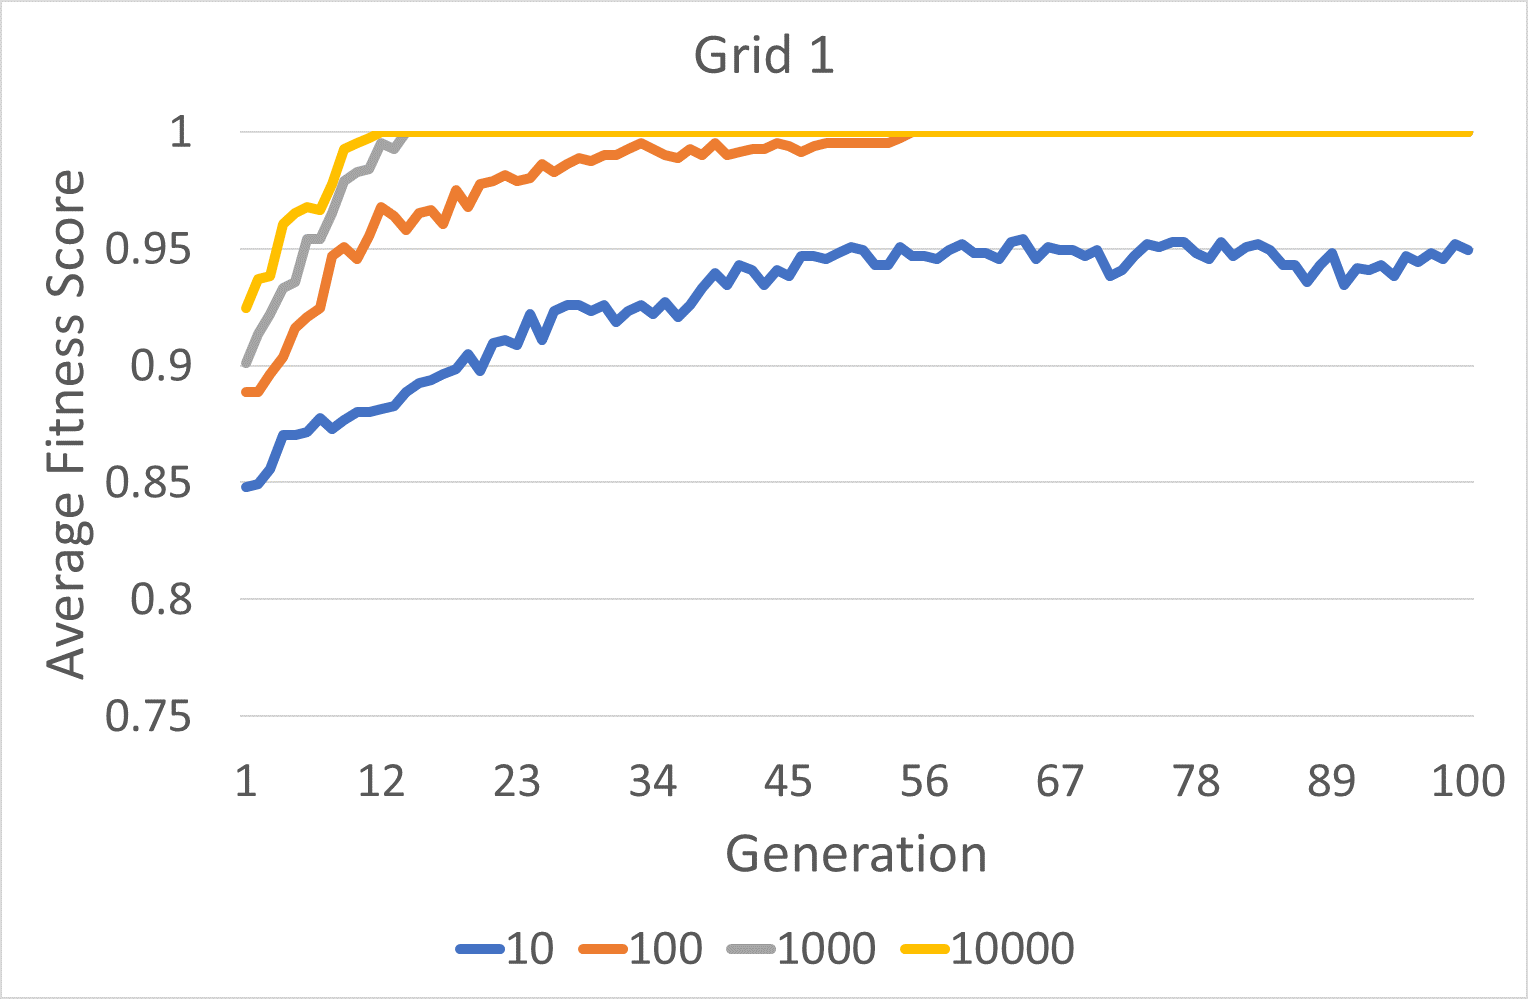
\includegraphics[width=.329\linewidth]{i/all_false_g1.png}\hfill
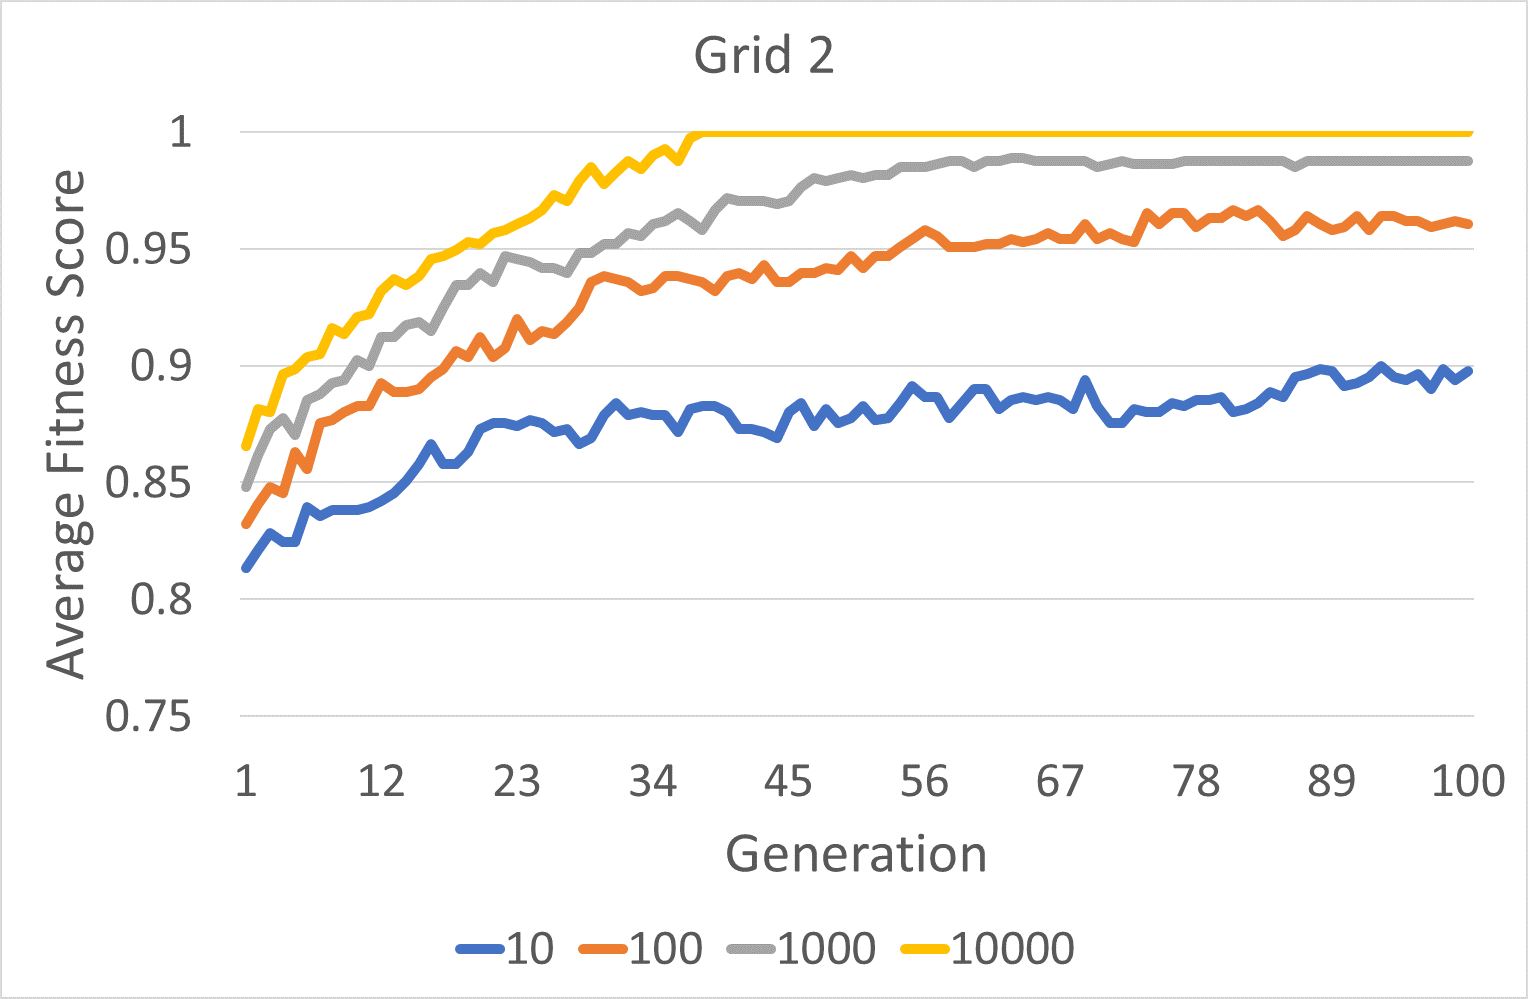
\includegraphics[width=.329\linewidth]{i/all_false_g2.png}\hfill
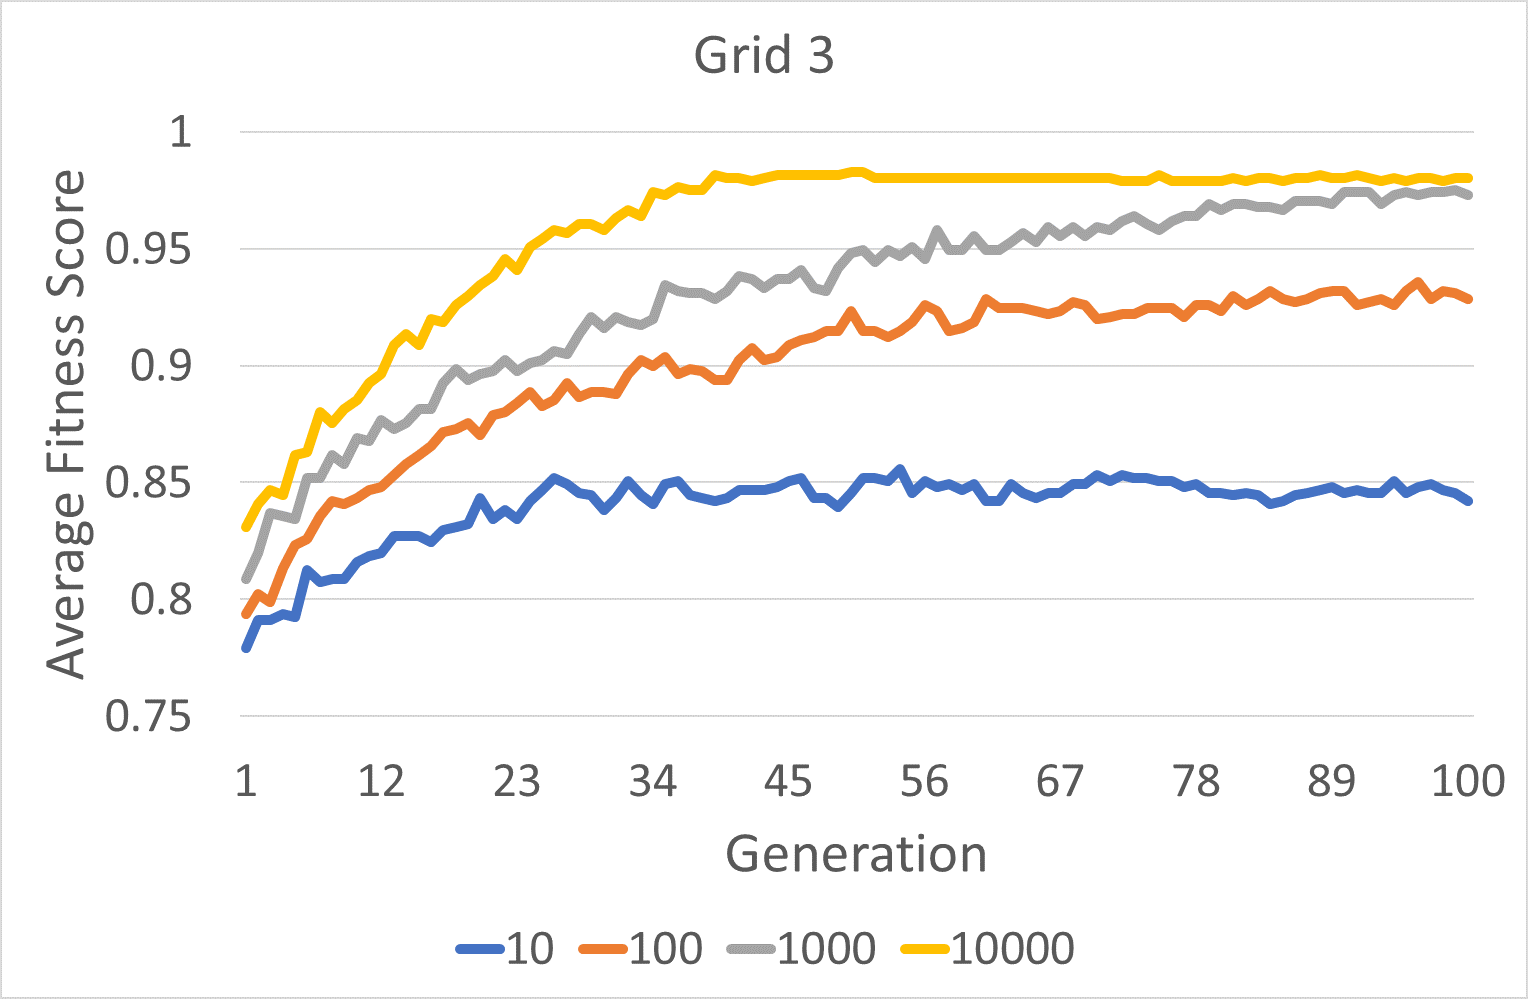
\includegraphics[width=.329\linewidth]{i/all_false_g3.png}

\caption{Results for the genetic algorithm with none of the advanced genetic operators applied. The fitness score is the average of five runs per population size over the sample set.}
\label{fig:all_false}

\end{figure}
\paragraph{•}

The first experiment run was to establish a baseline without any of the three modifications present and to show how both grid difficulty and population size affect the average fitness scores. In this experiment the tournament function operated as described in the design section without an implementation of the duel selector. The swap mutation was only carried out once and each subsequent generation replaced their parents entirely. This experiment was run on all three grids under each population size and the results of which can be seen in Figure \ref{fig:all_false}. The algorithm performed well on Grid 1 but its performance decreased on Grid 2 and Grid 3.
\paragraph{}
As expected, the largest population size of 10000 finds a solution in an average 13 generations and before other population sizes. However, the population of 1000 proved to be only slower by 4 generations, finding the solution in 17. Performance decreases as the difficulty increases with only the population of 10000 able to find a solution in all cases. On Grid 3, all of the population sizes plateau before finding the optimal solution. This is because while there is diversity of solutions produced between generations, there is no guarantee that the subsequent generation will be better than the current one. This is evident in the trend for some generations to experience a decrease in the maximum fitness value. This lack of stability in scores means that as the population begins to converge, there is a high chance that the population will begin to converge after the maximum fitness has decreased. Subsequently, the population starts to converge at a local maximum rather than the global maximum and a plateau forms.  

\begin{figure}[htp]

\centering
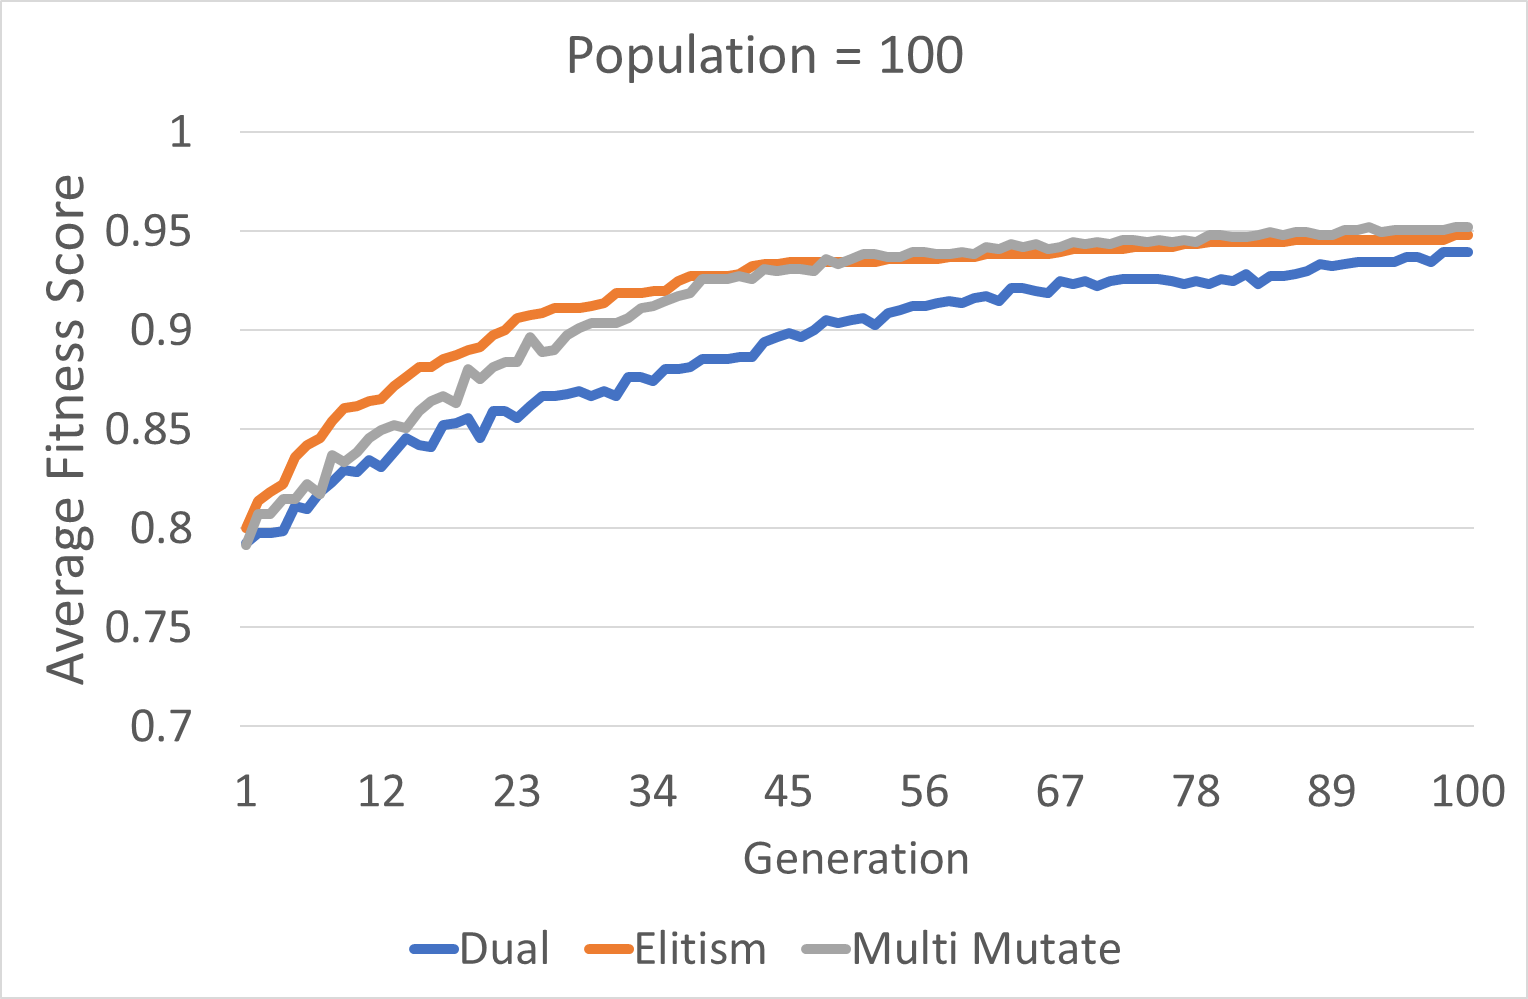
\includegraphics[width=.329\linewidth]{i/one_true_100.png}\hfill
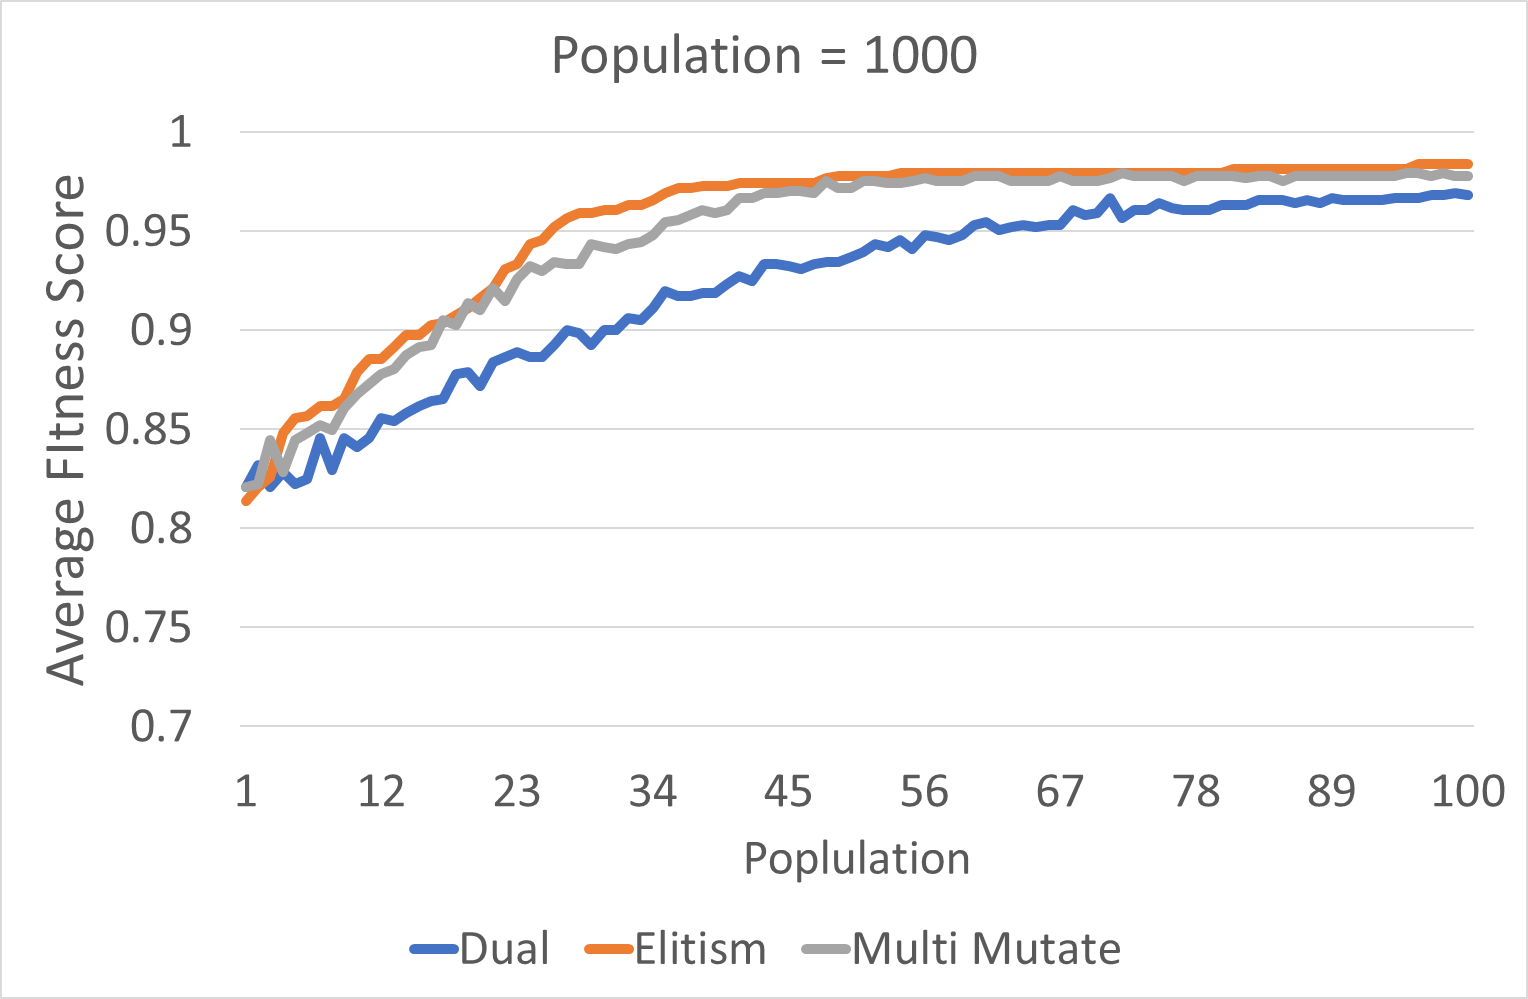
\includegraphics[width=.329\linewidth]{i/one_true_1000.png}\hfill
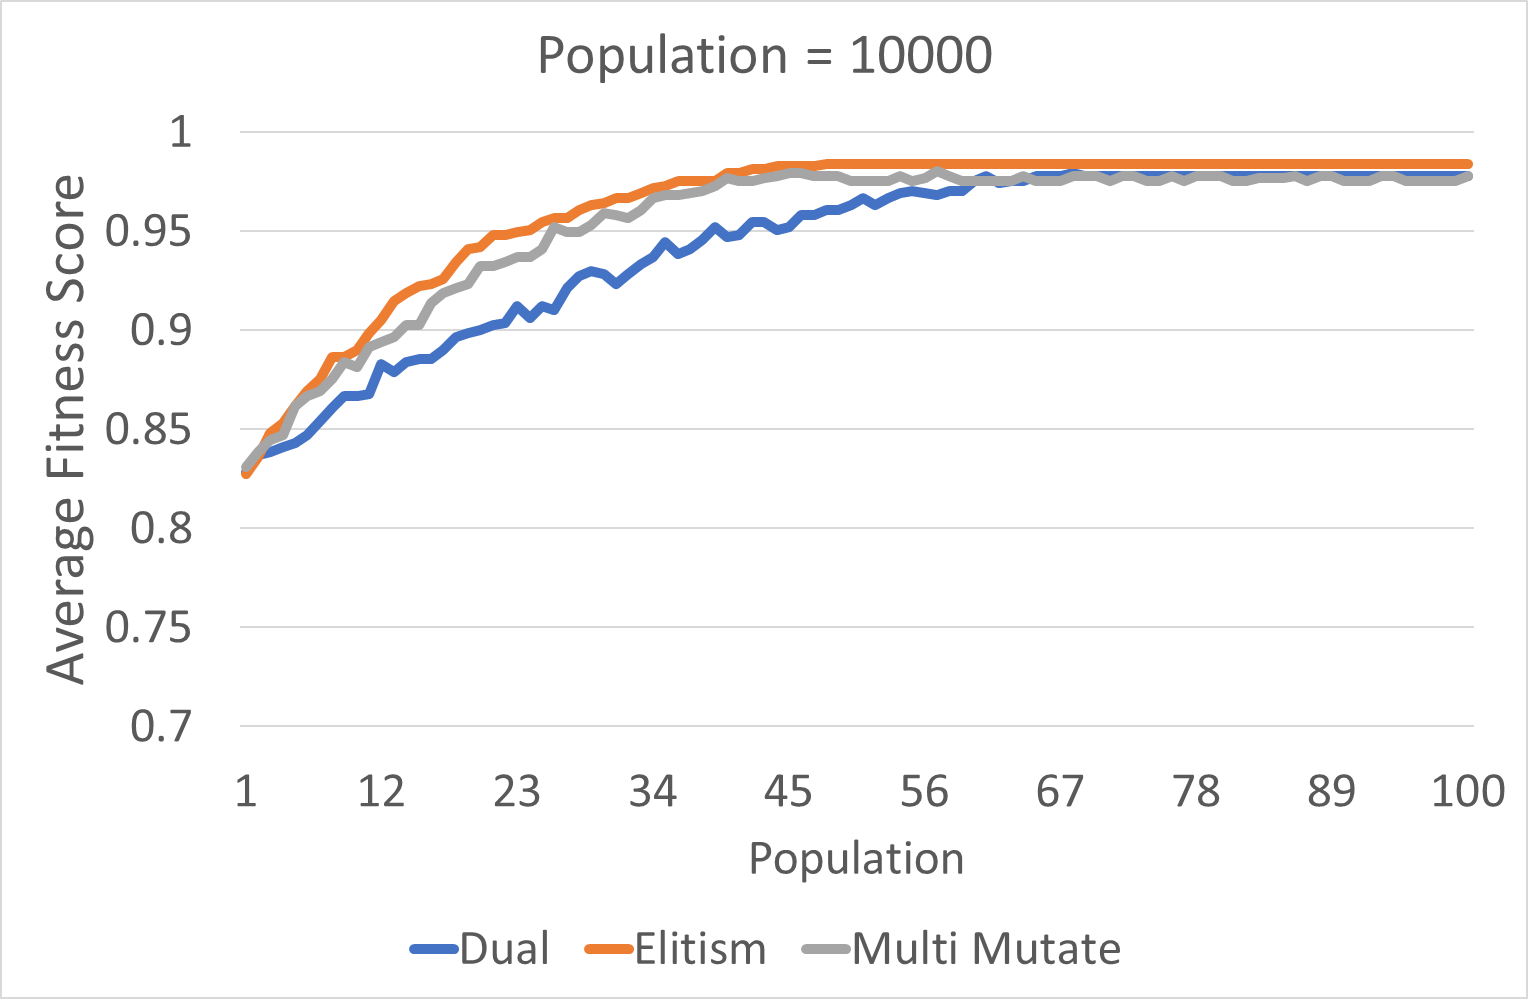
\includegraphics[width=.329\linewidth]{i/one_true_10000.png}

\caption{Results for the genetic algorithm with each of the advanced genetic operators applied. The fitness score is the average of five runs per population size when run on Grid 3.}
\label{fig:one_true}

\end{figure}

\paragraph{•}
The second experiment was run five times on populations of 100, 1000, and 1000 for one hundred generations with the aim of comparing the effect of duel selection, elitism and multi-mutation. Grid 3 was chosen for the experiment due to the poor performance shown in experiment one on the problem. The average fitness score measured at the end of each of one hundred generations is shown in Figure \ref{fig:one_true}. As the graphs show, in all cases adding the elitism operator to the genetic algorithm provided the greatest initial improvement in fitness scores between generations 1 and 45. Additionally, it reached the highest average fitness of the three operators at the end of one hundred generations. Initially, the multi-mutator operator lagged behind elitism due to the lower selection pressure not promoting individuals with a strong fitness. However, by one hundred generations the operator had reached a score comparable to that of those reached by the elitism operator. Both elitism and multi-mutation produced a higher average fitness score when compared against the same population for Grid 3 in experiment one. The genetic algorithm benefiting from both a stronger selection pressure and more solution diversity respectively. Duel selection lagged behind both of them due to the large decrease in selection pressure it affords populations which adversely affected the rate at which the population converged as well as the fitness score of the solution it converged to.


\begin{figure}[htp]

\centering
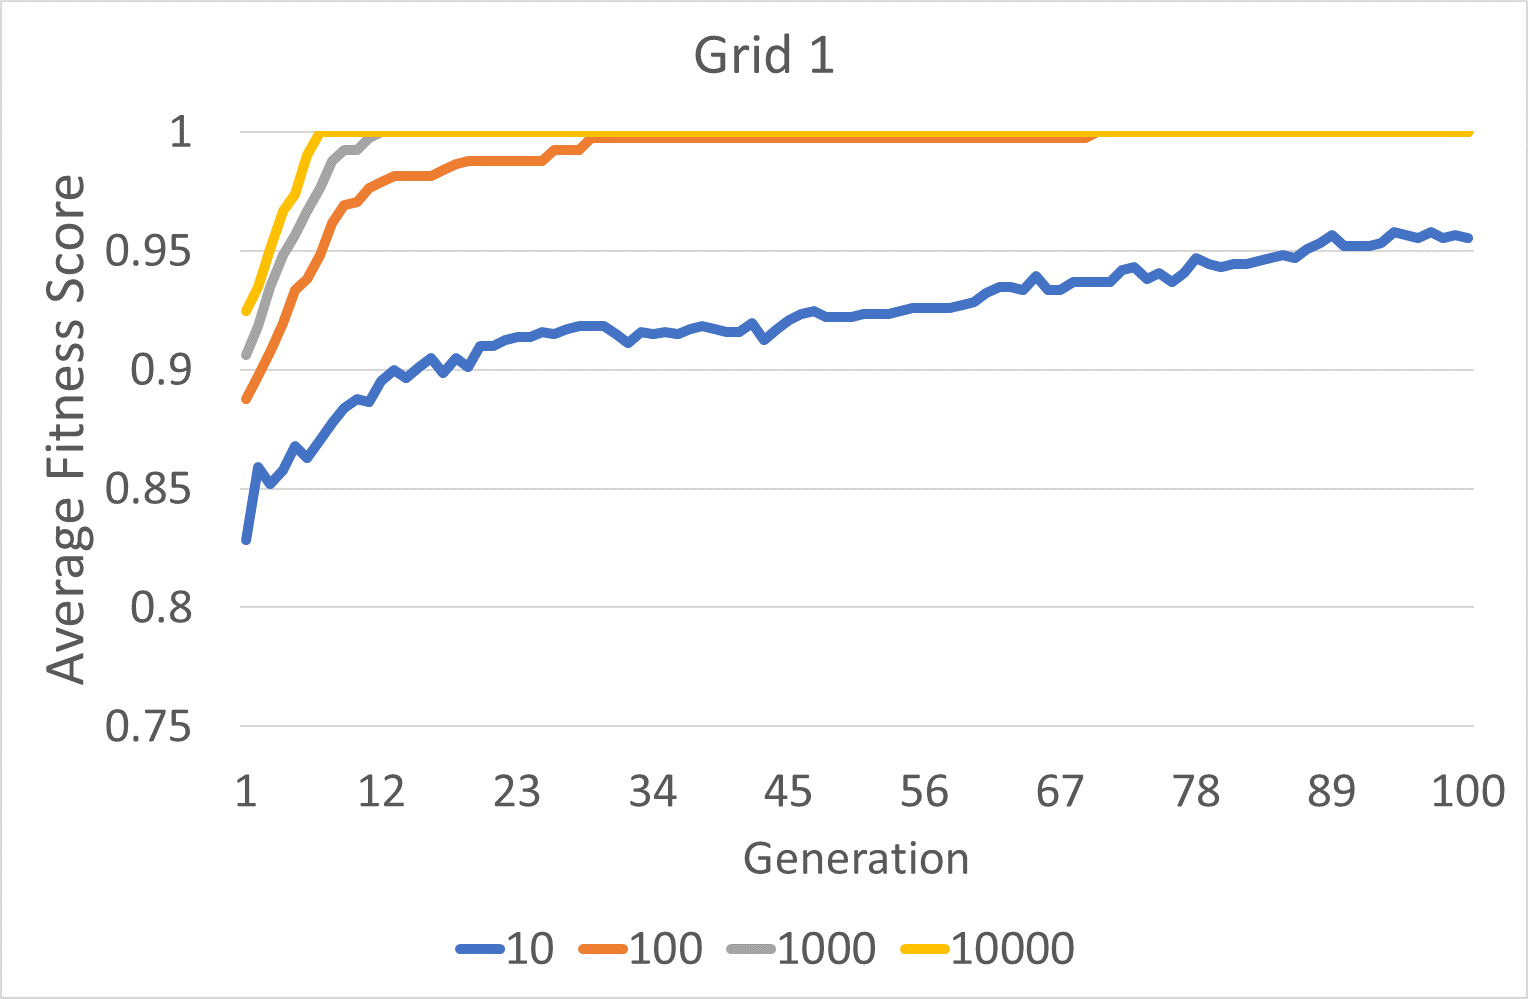
\includegraphics[width=.329\linewidth]{i/e_m_g1.png}\hfill
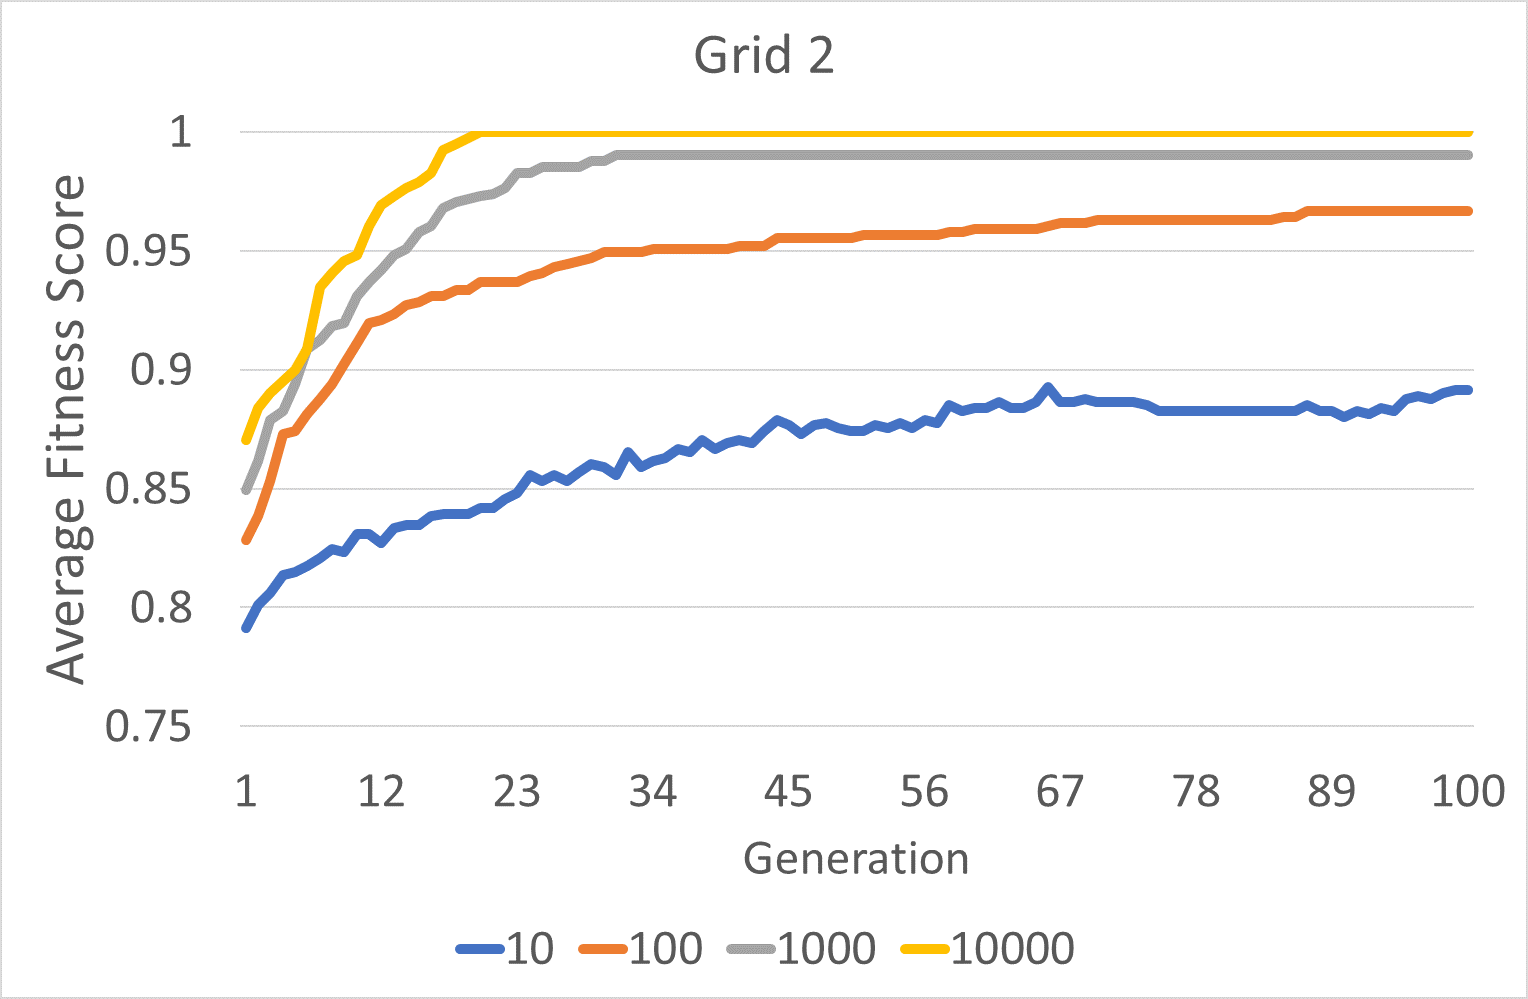
\includegraphics[width=.329\linewidth]{i/e_m_g2.png}\hfill
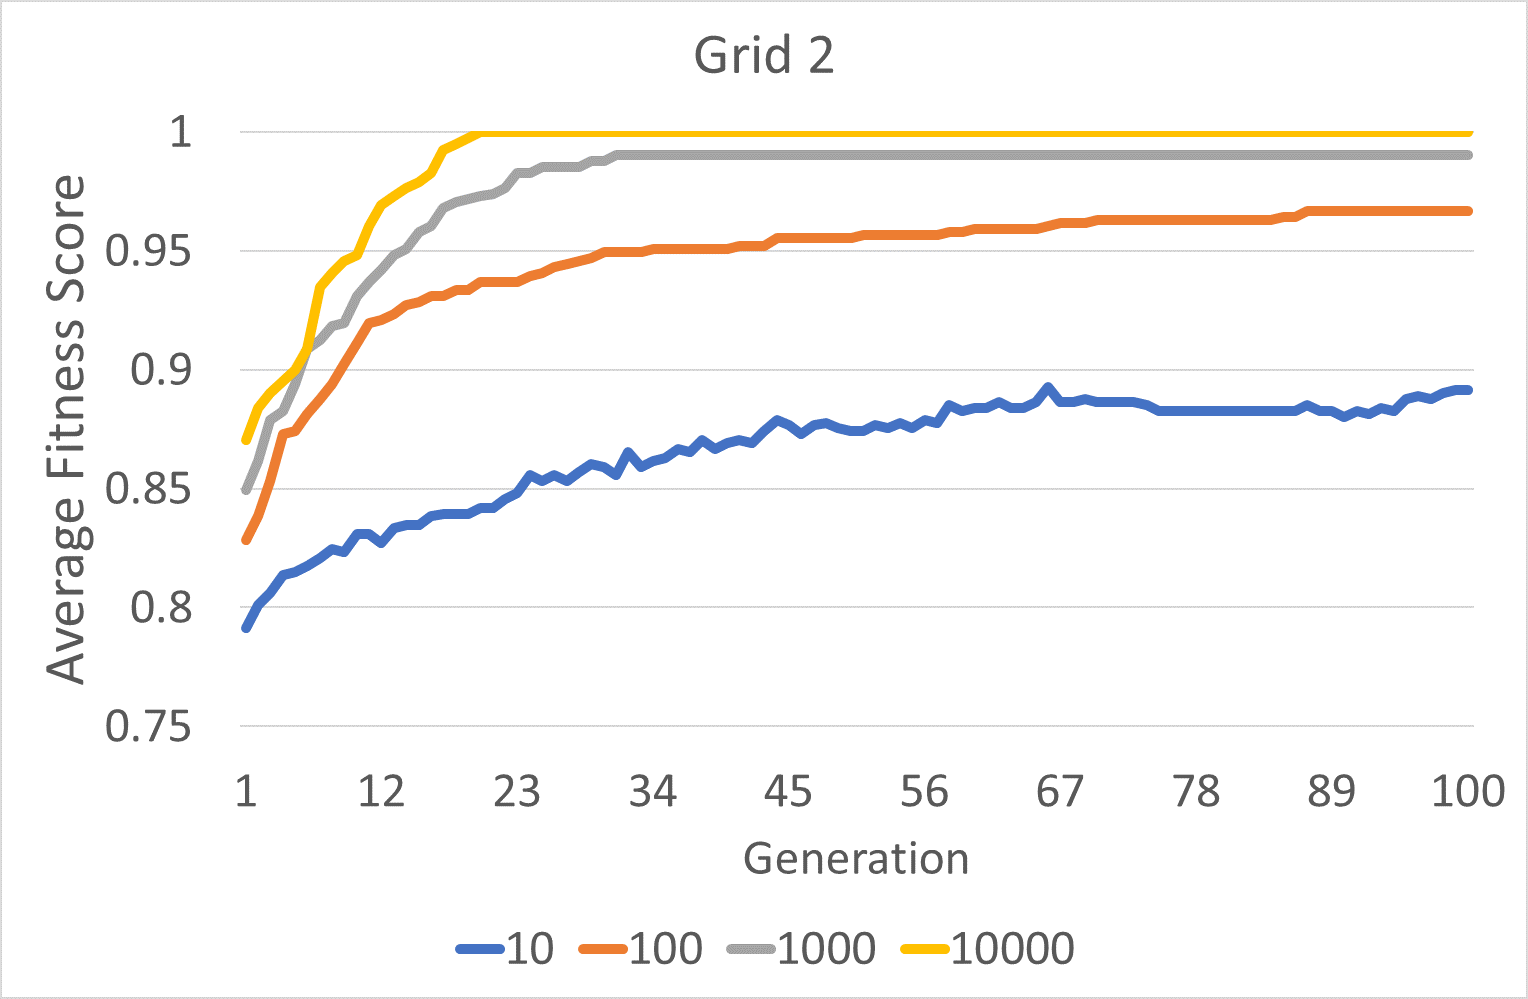
\includegraphics[width=.329\linewidth]{i/e_m_g3.png}

\caption{Results for the genetic algorithm with both elitism and multi-mutation genetic operators applied. The fitness score is the average of five runs per population size over the sample set.}
\label{fig:two_true}
\end{figure}

\paragraph{•}
Experiment three was initialised in the same way as experiment one but with the multi-mutation and elitism genetic operators applied. These genetic operators were selected because of the results shown in experiment two, where they both independently outperform both the genetic algorithm implemented in experiment one and the duel selection operator in experiment two. The experiment was designed in such a way because combining the two operators should provide move variety to the population of candidate solutions from using multi-mutation. When combined with the increased selection pressure from the elitism operator, candidate solutions with a high fitness score would be prioritised while those produced by multi-mutate which are significantly worse are discarded between generations. 
\paragraph{•}
As the results in Figure \ref{fig:two_true} show, the application of the two genetic operators has improved the average fitness score found on Grid 3 for a population of 10000 over that of experiment one. This is because, as hypothesised, the increase in diversity in the largest candidate pool allows for a larger chance that novel solutions will be produced that will lead away from a local maximum to that of a solution. When applied to Grid 1 the rate of increase did not improve for any population size due to both genetic algorithms finding the solution within ten to twenty generations for population sizes greater than ten. This is the greatest rate of increase possible using the row permutation initialisation and crossover methods described in the design section. For Grid 2, the new genetic algorithm found solutions on average ten generations faster than that of its predecessor. The elitism operator prevents the population 'moving backwards' when the average fitness score decreases between generations, thus increasing the rate of gain when applied to moderately difficult problems such as Grid 2.

\section{Questions}
\begin{enumerate}[label=(\alph*)]
\item The best population size was when the population equalled 10000 individuals.

\item As largest population, a population size of 10000 allowed for a pool of candidate solutions at least ten times larger than any other population. This increase in the candidate pool allowed for an increased amount of solution diversity within the pool, while still maintaining the same proportional selection pressure as the other population sizes. This meant that individuals which provide less optimal solutions but may lead to a solution over successive generations have a greater chance of remaining in the population. So too is the chance that these individuals will be generated, increasing the likelihood that the genetic algorithm will overcome a potential local maxima. This effect is compounded by the addition of multi-mutation in experiment three, which further increases the diversity of the candidate pool and slows the rate at which solutions within the population converge to a single value.

\item Grid 1 was the easiest while Grid 3 was the hardest.

\item Grid 1 was the easiest because the increased number of clues it contained reduced the search space that the algorithm was searching to find a solution while the smaller number of clues in Grid 3 caused the inverse. The addition of more clues also flattened the search space, reducing the number of local maxima. The clues helped 'guide' the algorithm towards the solution by removing the number of avenues it could evolve down which lead to a local maximum. When the number of clues decreased, then the search space became steeper, with the potential for the algorithm to find a solution which was close to the optimal fitness but would not lead to the true solution.

\item  A further experiment to be run would be one that would test the internal variables of the genetic algorithm, the mutation rate and the crossover rate. For each increment of 0.05 between 0 and 1 of the mutation rate, the same range of crossover rates should be tested. By repeating the runs five times and taking an average of the fitness functions for a range of populations, the optimal mutation and crossover rates would be found. This could be further enhanced by adding a third variable, the tournament size which would move the selector away from the current binary tournament configuration and to a true tournament selector. Another possible experiment would be to run the algorithm on a greater pool of Sudoku puzzles of varying difficulty such as twenty unique grids. Repeated five times with the average taken, these results can be compared against those of box and column permutation initialisation methods. This will test if the current row-based method could be replaced with a initialisation method which performs better over a greater number of Sudoku puzzles. 
\end{enumerate}

\end{document}
